\begin{song}{title=\predtitle\centering Racci\\\large Cermaque \& Iamme Candlewick  \vspace*{-0.3cm}}  %% sem se napíše jméno songu a autor
\begin{centerjustified}
    \vetsi
	
    ^{Emi \z}Tak dlouho volal racek ^{G}do prázdna,
    
    ^{Hmi \z}až z prázdna lásku ^*{\z A}přivola l,
    
    Ten příboj doplul sem až z dna,
    
    dva racci tančí u mola. \\\,\\
    
    
    Noc barví moře sametovou tuší,
    
    potom on vzlétne, ona netuší,
    
    zda už ji opustil,
    
    či pro ni hledá bezpečí. \\\,\\

    
    A vše je jedno, vše je dobře,
    
    že moře nikdy nemlčí.
    
    Ránu co nechá jedna vlna,
    
    vždy další vlna vyléčí. 

    
    \refren
    Já a ty, vlna za vlnou
    
    to moře mává křídly.
    
    Já a ty, vlna za vlnou
    
    to moře mává křídly.
    
    Já a ty, vlna za vlnou
    
    to moře mává křídly. \\\,\\
    
    
    Stařičký démon Poseidon
    
    vidlice místo obočí
    
    a v očích mořské propasti
    
    hlídá ať láska, nikdy neotročí.
    
    Ať vlna za vlnou
    
    nežene srdce do pastí. 
    
    
    \refren
    Já a ty, vlna za vlnou
    
    to moře mává křídly.
    
    Já a ty, vlna za vlnou
    
    to moře mává křídly.
    
    Já a ty, vlna za vlnou
    
    to moře mává křídly.
\end{centerjustified}

\newpage
\centering
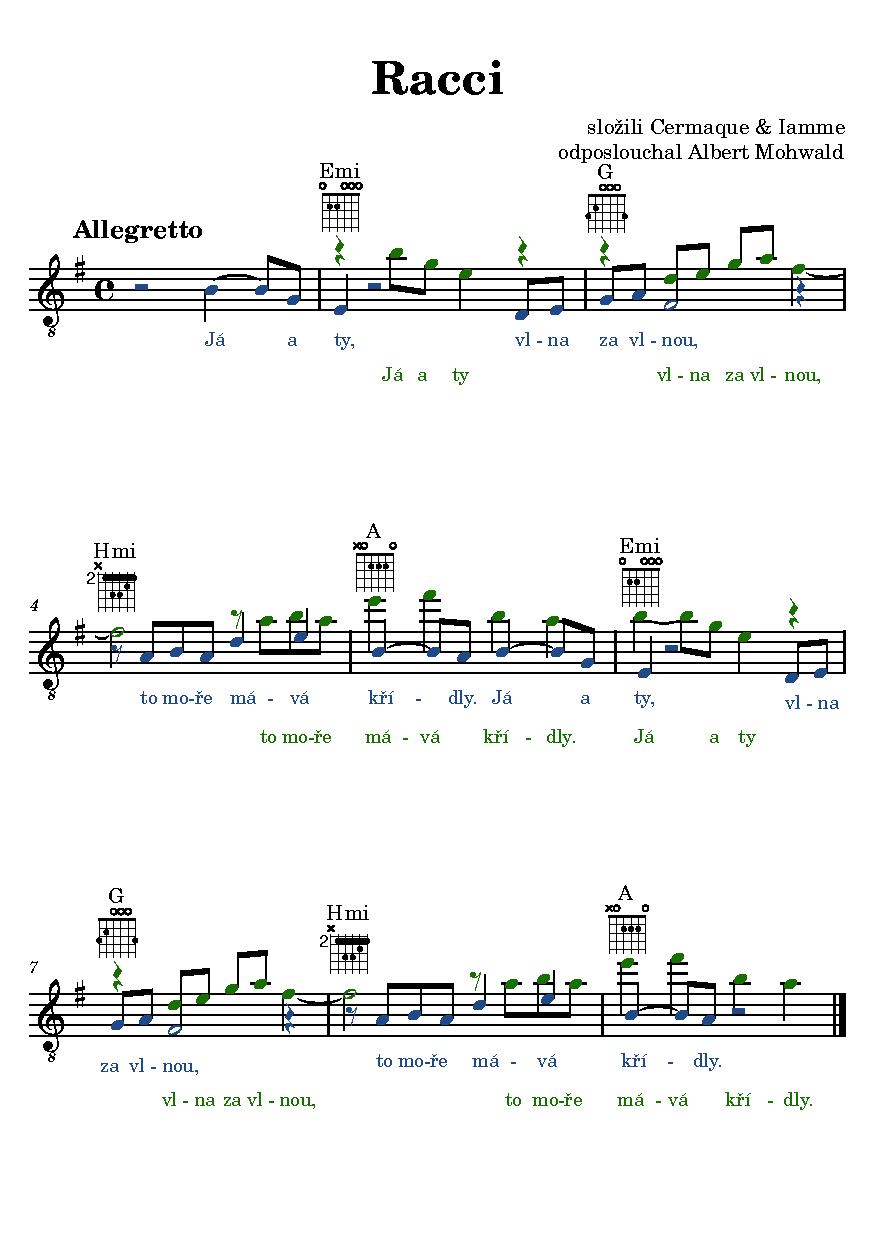
\includegraphics[scale=1.1]{../taby/racci-komplet.pdf}

\setcounter{Slokočet}{0}
\end{song}
